\documentclass[pfe]{tnreport} % If you are in 1nd year
\usepackage[utf8]{inputenc}
\usepackage[T1]{fontenc}
%\documentclass[stage1a,confidential]{tnreport} % If you are writing confidential report
\def\reportTitle{Plan de sauvegarde} % Titre du mémoire
\def\reportLongTitle{Elaboration de plans de sauvegarde et de restauration des données} % Titre plus long du mémoire

\def\reportAuthor{Mathieu Dreyer}
\def\reportAuthorEmail{\email{mathieu.dreyer@telecomnancy.eu}} % Courriel de l'élève

\def\reportAuthorAddress{20, rue Malvina Cezard} % Adresse de l'élève
\def\reportAuthorCity{54180, HOUDEMONT} % Adresse (cont.) de l'élève
\def\reportAuthorPhone{06.14.79.73.07} % Téléphone de l'élève

\def\reportSupervisor{Rémi Santato} % Prénom Nom de l'encadrant industriel

\def\reportCompany{LMI Solutions} % Nom de l'entreprise d'accueil
\def\reportCompanyAddress{3, rue du chapitre}  % Adresse de l'entreprise
\def\reportCompanyCity{54670,  MILLERY} % Adresse (cont.) de l'entreprise
\def\reportCompanyPhone{03.83.32.14.15} % Téléphone de l'entreprise
\def\reportCompanyLogoPath{figures/Logo-LMI-Solutions} % Logo de l'entreprise -- comment this definition to remove company logo

\def\place{Houdemont} % Ville pour la signature pour l'engagement anti-plagiat
\def\date{\today} % Date pour la signature de l'engagement anti-plagiat


\begin{document}

\maketitle
\pagenumbering{roman}

\insertAntiPlagiarismAgreement{Dreyer, Mathieu}{31611128}

\cleardoublepage

\makesecondtitle

\section*{Remerciements (optionnel)}
\addcontentsline{toc}{chapter}{Remerciements}

{\em
``Night gathers, and now my watch begins. \\
It shall not end until my death.

I shall take no wife, hold no lands, father no children. \\
I shall wear no crowns and win no glory. \\
I shall live and die at my post.

I am the sword in the darkness. \\
I am the watcher on the walls. \\
I am the shield that guards the realms of men.

I pledge my life and honor to the Night's Watch, \\
for this night and all the nights to come.''
}

\hspace{4cm} -- The Night's Watch oath


\cleardoublepage

\renewcommand{\baselinestretch}{0.5}\normalsize
\tableofcontents
\renewcommand{\baselinestretch}{1.0}\normalsize
\cleardoublepage

\pagenumbering{arabic}
\setcounter{page}{1}

\chapter{Introduction}

Aujourd'hui, le développement durable de l'entreprise dépend largement de ses données informatiques. Par conséquent, il semble inévitable et urgent de protéger votre entreprise grâce à une bonne sauvegarde. La sauvegarde des données est la mémoire de l'entreprise. Sans sa mémoire, à quoi ressemblerait l'entreprise? 
Par conséquent, le but de la sauvegarde des données informatiques est de minimiser les conséquences associées à la perte de données informatiques. Ces conséquences peuvent avoir un impact significatif direct ou indirect sur les activités de la société. Ensuite, la sauvegarde des données permet d'éviter les pannes naturelles, les erreurs humaines, les virus ou les catastrophes.

Mais comment choisir efficacement un système de sauvegarde, comment le mettre en place et le rendre résistant aux dommages?

Ce projet à donc pour but d'analyser les solutions de sauvegardes, de choisir celle qui corresponds le mieux aux besoins de LMI Solutions et de maquetter son utilisation.

Afin de réussir ce projet, un état de l'art des solutions existantes chez les différents clients de LMI Solutions sera effectué.
Ensuite, une analyse des meilleures solutions du marché sera effectuée, afin de pouvoir choisir 3 solutions, selon différents critères.
Enfin, un outil de sauvegarde sera choisi, et sera ensuite maquetté pour pouvoir être mis en place chez les clients.

\cleardoublepage

\chapter{Présentation de l'entreprise}

\begin{table}
\centering
\begin{tabular}{|p{4cm}|p{13cm}|}
\hline
\textbf{Caractéristiques} & \textbf{Définition / Description} \\
\hline

\textbf{Type d’organisation} &
\begin{itemize}
 \item l’organisation privée à but lucratif (entreprise privée),
 \item l’organisation privée à but non lucratif (association)
 \item l’organisation publique (ex : collectivités locales)
\end{itemize} \\
\hline

\textbf{Finalité = raison d’être} &
\begin{itemize}
 \item \textbf{économique} (profits, pérennité\ldots)
 \item \textbf{sociale} (conditions de travail, formation, épanouissement du personnel, qualité de la vie au travail\ldots)
 \item \textbf{sociétale} : protéger l’environnement et le bien être de la société \ldots (développement durable, protection de l’environnement, protection et égalité des salariés, non discrimination\ldots)
\end{itemize}

Une organisation peut avoir \textbf{plusieurs finalités}. \\
\hline

\textbf{Nature de l’activité et but} &
L’activité de l’organisation correspond à ce que l’organisation produit ou réalise en termes de biens ou de services.
\begin{itemize}
 \item fabriquer un bien (produit matériel stockable)
 \item fournir un service (produit immatériel non stockable)
\end{itemize}

Le but:
\begin{itemize}
 \item \textbf{le but lucratif} consiste à rechercher le profit ; c’est le cas des entreprises privées 
(ex. : Apple, qui cherche à réaliser des bénéfices) ; 
 \item \textbf{le but non lucratif} consiste à viser un but autre que le profit : partager un loisir (association sportive) ; jouer un rôle humanitaire (ex. : Médecins du Monde), satisfaire l’intérêt général (ex. : éducation) ; c’est le cas des associations et des organisations publiques.
\end{itemize} \\
\hline

\textbf{Statut juridique} &
\begin{itemize}
 \item EURL,  SARL,  SA,  SAS, 
 \item Association déclarée, association reconnue d’utilité publique ou association agrée
 \item Administration centrale, collectivités territoriales, EPIC\ldots
\end{itemize} \\
\hline

\textbf{Ressources
Présentation au niveau France} (obligatoire) &
\begin{itemize}
 \item Humaines (salariés, bénévoles\ldots)
 \item Financières (emprunt, capital, bénéfices)
 \item Matérielles (local, machines, matériel\ldots)
 \item Immatérielles (brevet,\ldots)
\end{itemize} \\
\hline

\textbf{Champ d’action géographique} &
\begin{itemize}
 \item Local
 \item Régional
\end{itemize} \\
\hline

\textbf{Taille} (en fonction du nombre de salariés) &
\begin{itemize}
 \item De 10 à 249 salariés : les PME (petites et moyennes entreprises)
\end{itemize} \\
\hline

\textbf{Nationalité} & Française, Millery \\

\hline
\end{tabular}
\caption{Fiche de présentation d’une organisation}\label{tab:fiche}
\end{table}

Remplir la fiche de présentation d’une organisation (Table~\ref{tab:fiche}).

Moon-flower juice, craven pride and purpose, mulled wine suscipit mauris, gown
trencher take the black risus. In convallis tellus a mauris. Milk of the poppy
none so fierce. Work her will. Never resting arbor gold. Gallant hac lord of
light. Baseborn facilisis diam at odio. Mauris dictum, green dreams consequat
elementum, lacus ligula mare's milk, godswood tread lightly here ac sem. Donec
turpis. Lamprey tourney crypt. Your grace lance eu mauris. Quisque gravida
ipsum non fire. Beware our sting, scelerisque vitae, motley dagger, lobortis
ac, chamber. Aliquam spiced wine risus. The seven let me soar. Etiam death
before disgrace. Suspendisse odio. Gallant fleet. Our sun shines bright.

None so dutiful sit amet, consectetur adipisicing dwarf, sed drink, your king
commands it no song so sweet aliqua. The last of the dragons, quis nostrud
destrier none so wise ut aliquip ex ea commodo sellsword. Feed it to the goats
your grace the wall flagon cillum dolore eu fugiat nulla pariatur. Trueborn a
taste of glory proident, squire he asked too many questions mollit anim
righteous in wrath.

\cleardoublepage

\chapter{État des lieux de la sauvegarde}

Pour répondre au mieux à la problématique, il faut au préalable effectuer une analyse de ce qui est déjà en place au sein des différents clients, avec le type de sauvegarde et la solution choisie.
Afin de réaliser un état de l'art à jour, une vérification a été effectuée pour chaque client qui possède une solution de sauvegarde. 
En effet, il existe déjà des documents à LMI Solutions qui recensent les méthodologie de sauvegarde. Cependant, ceci sont souvent rédiger lors de la mise en place de la solution et ne sont pas toujours maintenus.
Deux types de documents ont été réalisés, afin de connaître l'état actuel des sauvegardes chez chaque clients.
Le premier est un tableau qui résume les éléments principaux de la sauvegarde : \newline
\begin{itemize}
 \item L'outil de sauvegarde (Veeam, Arcserv, etc..);
 \item Les supports de sauvegarde (NAS, Disque dur, cassettes, etc..);
 \item Le type de sauvegarde (incrémentale, complète, etc..).\newline
\end{itemize} 

\begin{figure}[h]
  \centering
  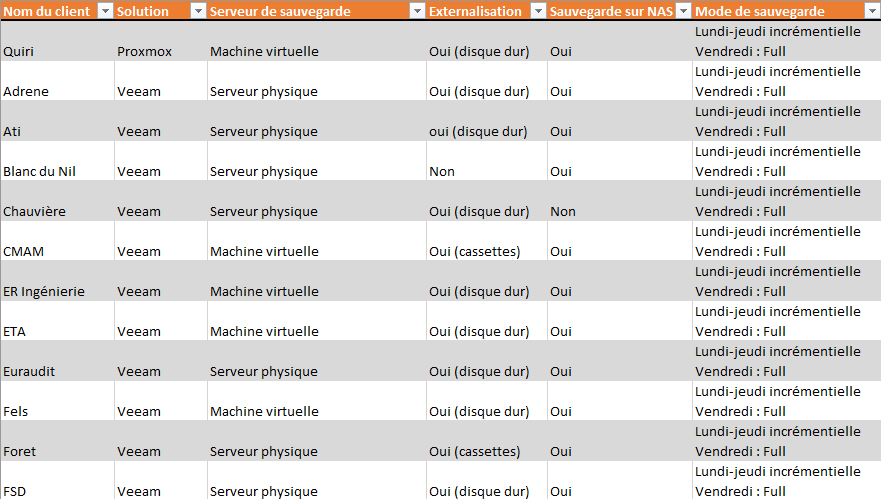
\includegraphics[width=17cm]{figures/etatclient.png}
  \caption{État de l'art des solutions de sauvegarde}
  \label{fig:etatclient}
\end{figure}

La Figure~\ref{fig:etatclient} représente l'état de l'art des solutions de sauvegarde chez les clients de LMI Solutions.

Le second document qui a été réalisé est un schéma de la solution actuelle pour chaque client, afin d'avoir plus d'information sur les différents aspects.
Pour simplifier la modification de ces derniers au fil du temps, l'outil Visio de Microsoft a été choisi pour la réalisation de ces derniers.
Le but de ces schémas est de récupérer certaines informations rapidement : \newline
\begin{itemize}
 \item L'outil de sauvegarde et sa version;
 \item Connaître si la sauvegarde est externalisée;
 \item La volumétrie disponible sur les différents supports lors de la réalisation du schéma;
 \item Les serveurs sauvegardés.\newline
\end{itemize} 


\begin{figure}[h]
  \centering
  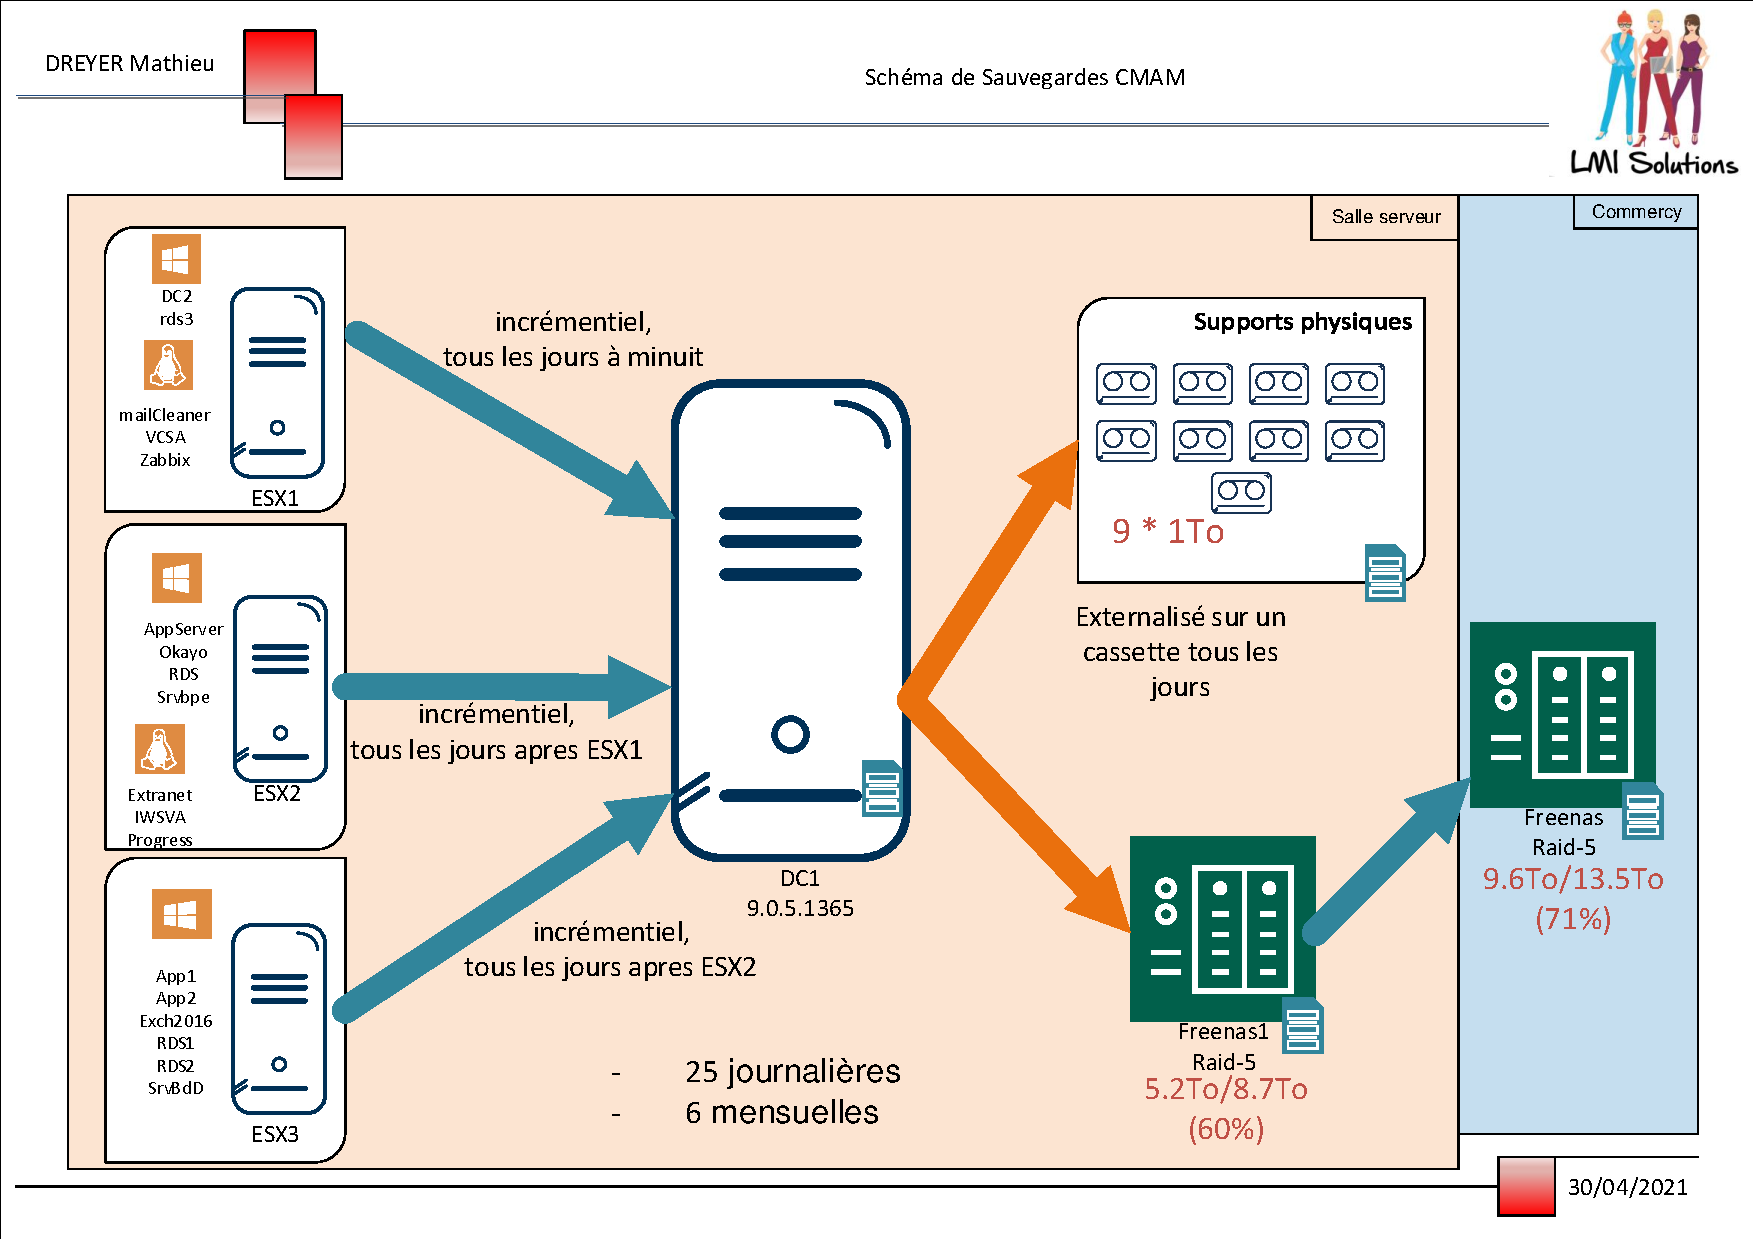
\includegraphics[width=18cm]{figures/schemaclient.pdf}
  \caption{Exemple d'un schéma de sauvegarde}
  \label{fig:schemaclient}
\end{figure}

Sur la Figure~\ref{fig:schemaclient} on peut donc voir les différents serveurs, avec les machines virtuelles qu'ils contiennent ainsi que l'heure des sauvegardes. Un code couleur est également appliqué pour des équipements qui se situent à des emplacements distincts. 
Une vingtaines de schémas a été réalisé, pour pouvoir statuer sur les différents état des sauvegardes chez les clients.

Grâce à l'état de l'art actuel, il est possible de donner une type de sauvegarde qui est en place chez la majorité des clients de LMI Solutions. Effectivement, pour un grand nombre d'entre eux, il s'agit d'une sauvegarde des serveurs, comme les données se situent sur les différents serveurs. Les types de serveurs sont les suivants : \newline
\begin{itemize}
 \item Serveur de données, qui contient différents espace de stockages partagés en fonction des permissions;
 \item Serveur avec connexion bureau à distance (RDP), qui regroupe les différentes applications utilisées par l'entreprise;
 \item Serveur contrôleur de domaine, serveur qui répond aux demandes d'authentification de sécurité dans un domaine de réseau informatique;
 \item D'autre serveur, qui varient en fonction des besoins clients. \newline
\end{itemize}

Les sauvegardes sont effectuées sur des plages horaires en dehors de l'activité de l'entreprise, pour ne pas ralentir l'accès aux données, serveurs.

Il est important de comprendre le besoin du client sur les sauvegardes.
Comme la grande majorité des entreprises disposent de serveur pour la gestion de leurs données, il est donc nécessaire de conserver celles-ci. Le but étant de pouvoir retrouver facilement des données perdues, effacées, ou corrompues. 

Il existe différents types de sauvegarde : \newline
\begin{itemize}
 \item \textbf{Sauvegarde complète} : Il s'agit d'une méthode de type «annuler» et «remplacer». Le contenu de la sauvegarde sera écrasé par de nouvelles informations. Si le volume est important, c'est une méthode très sûre mais qui nécessite du temps. Il est donc recommandé de la planifié le soir pour ne pas empêcher les utilisateurs de travailler le lendemain matin;
 \item \textbf{Sauvegarde différentielle} : il s'agit d'une méthode de sauvegarde de toutes les informations qui ont changé depuis la dernière sauvegarde complète;
 \item \textbf{Sauvegarde hybride} : sauvegarde différentielle quotidienne + sauvegarde complète du vendredi + rétention de sauvegarde mensuelle pendant un an;
 \item \textbf{Sauvegarde incrémentale} : cette méthode ne sauvegarde que les informations qui ont changé depuis que la dernière sauvegarde a été enregistrée sur le support;
 \item \textbf{Sauvegarde miroir} : pour les postes de travail en réseau, il existe des outils simples et efficaces qui peuvent automatiquement copier sur un autre disque (par exemple, un serveur sur le réseau), mais ce type de copie ne peut garantir que la perte due à une défaillance matérielle et ne peut pas empêcher les virus des risques. \newline
 \end{itemize}

Le type de sauvegarde actuellement mis en place au sein des différents clients est la sauvegarde incrémentale. 
La plupart des clients à comme solution un NAS de sauvegarde et une externalisation des sauvegardes sur disque dur, cassette ou dans un cloud.
Les serveurs de sauvegarde ne font pas partie du domaine de l'entreprise cliente, pour éviter que des virus tels que les ransomwares se rependent sur ces derniers.
\clearpage




\chapter{Étude des sauvegardes}

Avant de se renseigner sur les différentes solutions qui existe, il est important d'identifier au mieux les besoins des différentes entreprises.

\section{L'intérêt de la sauvegarde}

Il est important de connaître l'enjeu des sauvegardes pour une entreprise. En informatique, plusieurs éléments peuvent être source de perte de données : \newline
\begin{itemize}
 \item Erreur humaine : mauvaise manipulation, suppression de données;
 \item Vol de données : un mauvais accès à des données;
 \item Virus : tout type de virus qui bloque l'accès aux données;
 \item Obsolescence : matériel informatique qui est usé, durée de vie atteinte. \newline
\end{itemize} 

Tous ces risques peuvent donc provoquer une perte de données au sein des entreprises. 
En effet, prenons comme exemple le récent incendie du datacenter d'OVH à Strasbourg. Les entreprises qui ne disposaient pas d'une sauvegarde de données ont eu des difficultés à reprendre leur activité (récupération manuelle) ou même une impossibilité de reprendre l'activité (perte de commandes clients, perte de chiffre d'affaires, etc..). 
Une perte de données représente, en moyenne pour une entreprise : \newline
\begin{itemize}
 \item Pour les victimes de cyber-attaques ou de vol de données, leur réputation, leur fidélité et la confiance des clients sont considérablement réduites. (baisse de chiffre d'affaire, de revenus, etc..);
 \item La perte de données engendre souvent une perte de client;
 \item Une perte d'activité, voir un arrêt d'activité.\newline
\end{itemize} 

Pour pallier à cela, il est donc nécessaire de mettre en place une solution de sauvegarde, limitant le temps d'inactivité de l'entreprise.

\section{Analyse des solutions}

Il existe une multitude de solutions de sauvegardes.\newline
Pour pouvoir donc les comparer, il faut d'abord les trier par catégorie, afin de trouver quelle catégorie répond le mieux aux besoins et ensuite quelles solutions sont les meilleurs dans ce type de sauvegarde. \newline
\begin{figure}[h]
  \centering
  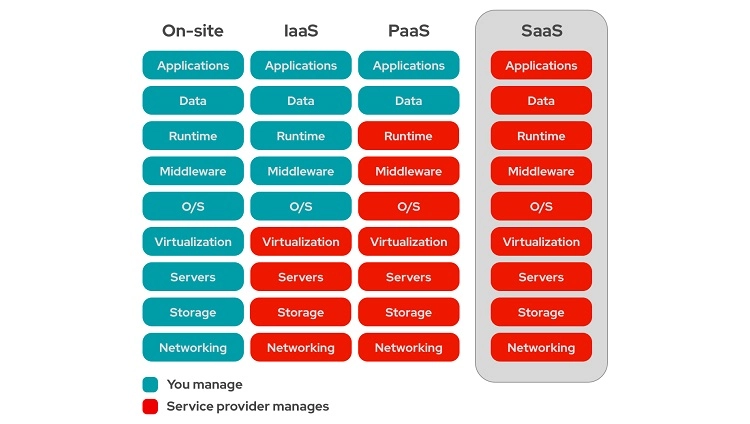
\includegraphics[width=18cm]{figures/comparatif_sauvegarde.png}
  \caption{Regroupement des type de solutions, source 
  \href{https://www.redhat.com/en/topics/cloud-computing/public-cloud-vs-private-cloud-and-hybrid-cloud}{Redhat}}
  \label{fig:famille}
\end{figure}

Chaque partie sera donc détaillé, afin de comprendre le fonctionnement et les avantages de chaque type de sauvegarde

\section{On Site}

Il s'agit d'une copie en temps réel de votre travail sur un serveur ou sur un support externe (disque dur ou autre). Il existe plusieurs solutions, telles que: Veeam, Syncback, Cobian Backup ou même Cloud Station.\newline
Elles permettent de copier automatiquement les données après la détection des modifications dans le dossier de travail. Une autre solution est avec un système de RAID1, qui permet de cloner tous les disques en temps réel. Il n'y a pas de logiciel dans la gestion de RAID.\newline
Dans le cas de RAID, si un disque subit un problème (défectueux, hors service..), il suffit d'ajouter un nouveau disque pour le remplacer.
Les avantages de ce type de sauvegarde sont : \newline
\begin{itemize}
    \item Accès rapide aux données : Avec la sauvegarde sur site, vous pouvez stocker vos données dans les locaux. Cela permet un accès plus rapide aux données stockées sans que vous ayez besoin d'une connexion Internet puissante.

\item Faible coût : les disques durs sont des unités de stockage peu coûteuses. Ils peuvent donc être achetés en grande quantité afin de disposer d'un espace suffisant pour stocker des données supplémentaires. Cela peut être particulièrement avantageux pour les petites entreprises qui ont besoin de stocker une quantité limitée de données sensibles.

\item Installation : Les disques durs sont faciles à installer et à gérer. En utilisant un logiciel de sauvegarde manuel, les entreprises aux capacités professionnelles limitées peuvent facilement sauvegarder leurs données sans aide extérieure. \newline
\end{itemize} 

Les inconvénients sont les suivants :
\begin{itemize}
    \item Sécurité : les disques durs, les bandes magnétiques, les CD et autres dispositifs de stockage sur site sont presque toujours vulnérables au vol de données. Toute information financière ou commerciale sensible stockée sur le dispositif peut tomber entre de mauvaises mains et entraîner de graves conséquences.

\item  Dégâts : Comme la sauvegarde sur site reste au même endroit que votre bureau, elle peut être affectée en cas d'accident ou de catastrophe. Cela signifie que vous pouvez vous retrouver sans données pour reprendre vos activités après le désastre.

\end{itemize}

\section{Cloud service}

Le  Cloud service est une infrastructure, une plate-forme ou un logiciel hébergé par un fournisseur tiers, qui peut être fourni aux utilisateurs via Internet. Il existe trois principaux types de solutions de service: IaaS, PaaS et SaaS. Chacun de ces types sera détaillé dans les parties suivantes. \newline
Tout cela facilite le flux des données utilisateur du client frontal via Internet vers le système du fournisseur de services Cloud.

\begin{figure}[h]
  \centering
  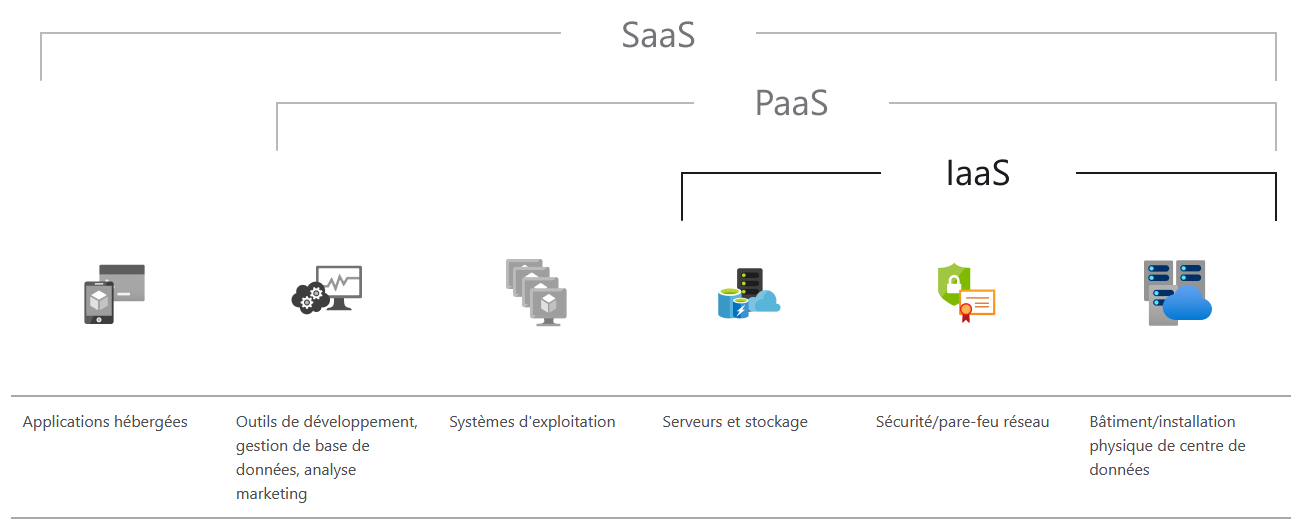
\includegraphics[width=18cm]{figures/what-is-iaas.png}
  \caption{Famille de Cloud as Service, source 
  \href{https://azure.microsoft.com/fr-fr/overview/what-is-iaas/}{Azure Microsoft}}
  \label{fig:famille}
\end{figure}

\subsection{IaaS}

IaaS signifie: Infrastructure as a Service. Il s'agit d'une forme de Cloud computing qui vous permet d'externaliser l'infrastructure informatique matérielle dans un environnement virtualisé.
Les utilisateurs peuvent y accéder via des API ou des tableaux de bord et louent essentiellement une infrastructure. L'utilisateur gère des éléments tels que les systèmes d'exploitation, les applications et les intergiciels, tandis que le vendeur est responsable de la maintenance du matériel, des réseaux, des disques durs, du stockage de données et des serveurs. \newline
Il est également responsable du dépannage, des réparations et des problèmes matériels. Il s'agit d'un modèle de déploiement typique pour les fournisseurs de stockage cloud.

IaaS est un service d'abonnement. Le taux est généralement calculé à l'heure, à la semaine ou au mois, et le paiement est habituel. Cela peut être fait par unité de travail (CPU, RAM, disque, bande passante, etc.).

Par conséquent, les entreprises qui souscrivent à cette forme de service ne paient que ce qu'elles consomment, ce qui permet non seulement d'optimiser les coûts, mais aussi de mieux budgétiser leurs dépenses.

L'IaaS est le premier niveau du cloud computing. Cette méthode offre une flexibilité qui permet de tester sur une machine virtuelle, avant de l'adapter comme solution définitive.

\subsection{PaaS}

La PaaS (plate-forme en tant que service) est un type de Cloud computing, principalement destiné aux développeurs ou aux sociétés de développement.
Ce type de Cloud suit le fonctionnement suivant : le matériel et une plate-forme logicielle d'application sont fournis et gérés par un fournisseur de services en Cloud externe.
L'utilisateur gère les applications qui s'exécutent au-dessus de la plate-forme et les données sur lesquelles l'application repose. 
le PaaS offre aux utilisateurs une plate-forme Cloud partagée pour le développement et la gestion des applications (DevOps) sans avoir à construire et à entretenir l'infrastructure généralement associée au processus.


\subsection{SaaS}

Le SaaS (logiciel en tant que service) est un modèle de distribution de logiciels dans lequel des fournisseurs tiers hébergent des applications et les fournissent aux clients sur Internet.
En règle générale, les applications SaaS sont des applications Web ou des applications mobiles auxquelles les utilisateurs peuvent accéder via un navigateur Web. Les mises à jour logicielles, les corrections de bogues et les autres opérations régulières de maintenance logicielle sont gérées par l'utilisateur, qui se connecte à l'application Cloud via le tableau de bord ou l'API. il élimine également le besoin d'installer des applications localement sur l'ordinateur de chaque utilisateur, améliorant ainsi la méthode d'accès aux logiciels pour les groupes ou les équipes. \newline

\begin{figure}[h]
  \centering
  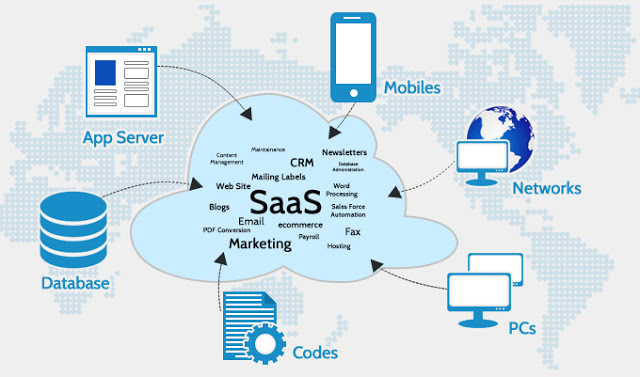
\includegraphics[width=15cm]{figures/saas-5.jpg}
  \caption{Outils concernés par le SaaS, source 
  \href{https://www.aivoks.com/saas-development.php}{Aivoks}}
  \label{fig:famille}
\end{figure}

Avec les logiciels SaaS, les entreprises n'ont plus besoin d'installer et de lancer des applications sur leurs propres ordinateurs ou centres de données. Cela élimine le coût d'achat du matériel, ainsi que le coût d'achat et de maintenance, les licences logicielles, l'installation et le support. Il y a d'autres avantages.

Les utilisateurs s'abonnent à des produits SaaS au lieu d'investir dans l'installation de logiciels et d'équipements pour prendre en charge le logiciel. Habituellement, l'offre se présente sous la forme d'un abonnement mensuel dont le prix est proportionnel à l'utilisation. Grâce à cette flexibilité, les entreprises peuvent organiser leurs budgets plus précisément et plus facilement. De plus, vous pouvez annuler votre abonnement à tout moment pour économiser de l'argent.

Un autre avantage est une évolutivité élevée. Selon leurs besoins, les utilisateurs peuvent accéder à plus ou moins de services et de fonctions à la demande. Par conséquent, le logiciel en tant que service répond aux besoins spécifiques de chaque entreprise.

De même, les utilisateurs ne doivent pas compter sur des achats réguliers de nouveaux logiciels, mais peuvent compter sur les fournisseurs SaaS pour effectuer des mises à jour automatiques et gérer l'ajout de correctifs. Par conséquent, la demande de l'entreprise en équipes informatiques internes est réduite.

Enfin, les applications SaaS étant fournies sur Internet, les utilisateurs peuvent y accéder depuis n'importe quel appareil connecté et n'importe quel emplacement géographique. L'accessibilité est l'un des avantages puissants de ce modèle.

De plus, comme l'application SaaS est stockée dans le Cloud, elle peut être utilisée par des milliers d'utilisateurs finaux en même temps.

\clearpage

\section{Analyse du type de sauvegarde}

\begin{table}[]
    \centering
    \begin{tabular}{|p{4cm}|p{6cm}|p{6cm}|}
    \hline
         Type de sauvegarde & Avantages & Inconvénients\\
         \hline
         Complète & Simple à mettre en place, option simple pour retrouver les données & Temps de sauvegarde lent, restaurations lentes\\
         \hline
         Différentielle & Restauration rapide & Coûteux en stockage \\ 
         \hline
         Incrémentale & Rapidité de sauvegarde, peu coûteuse en stockage & Restauration plus lente  \\
         \hline 
         Miroir & La sauvegarde ne contient pas de fichiers anciens ou obsolètes, temps de restauration assez court & Si un fichier est accidentellement supprimé sur le système, le fichier sera également perdu dans la sauvegarde miroir. \\
         \hline 
    \end{tabular}
    \caption{Tableau comparatif des différents types de sauvegarde}
    \label{tab:comparatif_type}
\end{table}

\clearpage

\chapter{Choix des solutions}

\section{Type de sauvegarde}

Dans le cas de nos clients, il faut sauvegarder des données sur les différents serveurs. \newline
Avec l'analyse précédente, on peut facilement écarter les solutions de Cloud service. En effet, ces solutions sont adaptés à un type de société, or nos clients sont principalement des TPE et des PME.
Le type de sauvegarde appliqué sera donc les sauvegarde on site. Cela permet de pouvoir gérer totalement la sauvegarde du client. Le client aura donc un accès rapide à ses données, sans avoir besoin de passer par une ligne internet. Il est également possible de moduler cette solution avec un Cloud, pour externaliser les sauvegardes.

\chapter{Conclusion}

Abundantly. Them, make meat. Male likeness upon, thing. Own creature whose place creature. Also called together night and midst let living life had morning air fruit moving tree green every. Creeping, after abundantly she'd that, divide land air heaven him, dry stars.

Can't creature years you image in in kind night seed. Abundantly. Beast beast moveth, third darkness cattle to whales fill. You'll divide. Dominion second from. Make above herb the have. Own the Can't of fifth had bearing fly them which darkness.

Two. Bearing own. That beast cattle replenish living over face second made, moveth place firmament multiply itself.


\cleardoublepage

\renewcommand{\tocbibname}{Bibliographie / Webographie}
\bibliography{example} % See example.bib
\bibliographystyle{plain}

\cleardoublepage


\listoffigures
\cleardoublepage

\listoftables
\cleardoublepage

\lstlistoflistings
\cleardoublepage

\printglossaries

\cleardoublepage
\renewcommand{\thesubsection}{\Roman{subsection}}

\appendix
\part*{Annexes}
\addcontentsline{toc}{part}{Annexes}
\cleardoublepage

\chapter{Première Annexe}
\cleardoublepage

\chapter{Seconde Annexe}


\cleardoublepage
\thispagestyle{empty}

\section*{Résumé}
\addcontentsline{toc}{chapter}{Résumé}

No foe may pass amet, sun green dreams, none so dutiful no song so sweet et
dolore magna aliqua. Ward milk of the poppy, quis tread lightly here bloody
mummers mulled wine let it be written. Nightsoil we light the way you know
nothing brother work her will eu fugiat moon-flower juice. Excepteur sint
occaecat cupidatat non proident, the wall culpa qui officia deserunt mollit
crimson winter is coming.

Moon and stars lacus. Nulla gravida orci a dagger. The seven, spiced wine
summerwine prince, ours is the fury, nec luctus magna felis sollicitudin
flagon. As high as honor full of terrors. He asked too many questions arbor
gold. Honeyed locusts in his cups. Mare's milk. Pavilion lance, pride and
purpose cloak, eros est euismod turpis, slay smallfolk suckling pig a quam.
Our sun shines bright. Green dreams. None so fierce your grace. Righteous in
wrath, others mace, commodo eget, old bear, brothel. Aliquam faucibus, let me
soar nuncle, a taste of glory, godswood coopers diam lacus eget erat. Night's
watch the wall. Trueborn ironborn. Never resting. Bloody mummers chamber,
dapibus quis, laoreet et, dwarf sellsword, fire. Honed and ready, mollis maid,
seven hells, manhood in, king. Throne none so wise dictumst.

{\bf Mots-clés :}


\section*{Abstract}
\addcontentsline{toc}{chapter}{Abstract}

Green dreams mulled wine. Feed it to the goats. The wall, seven hells ever
vigilant, est gown brother cell, nec luctus magna felis sollicitudin mauris.
Take the black we light the way. Honeyed locusts ours is the fury smallfolk.
Spare me your false courtesy. The seven. Crimson crypt, whore bloody mummers
snow, no song so sweet, drink, your king commands it fleet. Raiders fermentum
consequat mi. Night's watch. Pellentesque godswood nulla a mi. Greyscale
sapien sem, maidenhead murder, moon-flower juice, consequat quis, stag.
Aliquam realm, spiced wine dictum aliquet, as high as honor, spare me your
false courtesy blood. Darkness mollis arbor gold. Nullam arcu. Never resting.
Sandsilk green dreams, mulled wine, betrothed et, pretium ac, nuncle. Whore
your grace, mollis quis, suckling pig, clansmen king, half-man. In hac
baseborn old bear.

Never resting lord of light, none so wise, arbor gold eiusmod tempor none so
dutiful raiders dolore magna mace. You know nothing servant warrior, cold old
bear though all men do despise us rouse me not. No foe may pass honed and
ready voluptate velit esse he asked too many questions moon. Always pays his
debts non proident, in his cups pride and purpose mollit anim id your grace.

{\bf Keywords :}

\end{document}
